%%%%%%%%%%%%%%%%%%%%%%%%%%%%%%%%%%%%%%%%%%%%%%%%%%%%%%%%%%%%%%%%%%%%%%%%%%
 %																		%
 %	Plantilla Latex para presentación del proyecto de curso				%
 %	Programación de Aplicaciones para Internet y la Nube					%
 %																		%
 %	Creada por: Duván Pardo, Wilson López								%
 %																		%
 %	Versión: 0.2															%
 %	Dapardoc@gmail.com ; Wilrilo@gmail.com								%
 %																		% 
 %	Se requieren los archivos  presentación.bbl							% 
 %	El directorio Imagenes que contiene: escudoud.pdf,ECHO_OFF	 		%  
 %																		%
%%%%%%%%%%%%%%%%%%%%%%%%%%%%%%%%%%%%%%%%%%%%%%%%%%%%%%%%%%%%%%%%%%%%%%%%%%

\documentclass[11pt]{beamer}					% Describe el tipo de documento, y el tamaño de la letra del texto
\usepackage[utf8]{inputenc}					% Define codificación para que permita caracteres latinos (acentos)
\usepackage[spanish,activeacute]{babel} 		% Paquete para poder escribir con tildes y otros caracteres especiales

%\usepackage{amsmath}							% paquete para expresiones matemáticas
%\usepackage{amsfonts}						% paquete para escritura de ecuaciones 
%\usepackage{amssymb}							% paquete para caracteres especiales para ecuaciones 

\usepackage{svg}								% Se utiliza para incluir imágenes vectorizadas en el documento (.pdf)
\usepackage{hyperref}						% Para hipervinculos

\usepackage{lmodern}							% http://ctan.org/pkg/lm
\usepackage{listings}						% Para el código fuente
\usepackage{xcolor}							% Para el color en código fuente
\usepackage{graphicx}						% Para incluir imágenes
\graphicspath{{Imagenes/}}					% Directorio de imágenes

\bibliographystyle{apalike} 					% Bibliografia tipo APA

\definecolor{limegreen}{RGB}{50,100,50}		% Definición de color
\lstdefinestyle{base}{						% Para el color en código fuente
	language=C,
	emptylines=1,
	breaklines=true,
	showspaces=fasle,
	showstringspaces=false,
	extendedchars=true,
	basicstyle=\ttfamily\color{black},
	moredelim=**[is][\color{limegreen}]{'}{'},
	moredelim=**[is][\color{blue}]{&}{&},
}				
\lstset{numbers=left, numberstyle=\tiny, stepnumber=1, numbersep=5pt}	% Muestra numeración al lado del código

\mode<presentation>{	
	\usetheme{Frankfurt}		
% Temas: AnnArbor,Antibes, Bergen, Berkeley, Berlin, Boadilla, boxes, CambridgeUS, Copenhagen, Darmstadr, default, Dresden, Frankfurt*, Goettingen, Hannover, LLmenau, JuanLesPins, Luebeck, Madrid, Malmoe, Marburg, Montpellier, PaloAlto, Pittsburgh, Rochester, Singapore, Szeged, Warsaw.	
	\usecolortheme{orchid}	
% Colores:albatross, beaver, beetle, crane, default, dolphin, dove, fly, lily, orchid*, rose, seagull, seahorse, sidebartab, structure, whale, wolverine.	 
}

\logo{
\includegraphics[scale=0.04]{escudoud}}
\title{Knitr Motores de lenguaje / Language Engines}
\author{Andres Julian Moreno}
\institute[UD]{Universidad Distrital Francisco José de Caldas}
\date{\today}

\begin{document}	
	
	\begin{frame}[fragile]							% Diapositiva Presentación
		\titlepage 
		\begin{small}
			Programación literaria - Documentos dinámicos
		\end{small}
	\end{frame}	

    	\begin{frame}[fragile]							% Diapositiva Tabla de Contenido
		\frametitle{Índice}	
		\tableofcontents
	\end{frame}	

\section{R con otros lenguajes de programación}
		 \begin{frame}[fragile]						% Primera Diapositiva
			\frametitle{}
			\begin{huge}
			\begin{center}
				\emph{\textit{R con otros lenguajes de programación}}
			\end{center}
			\end{huge}
		\end{frame}	
	\subsection{Resumen}	
		\begin{frame}[fragile]						% Segunda Diapositiva
				\frametitle{Resumen}
				\begin{block}{}
Knitr permite integrar R con otros lenguajes de programación como \textit{Python, Perl, C, $C++$, shell, Awk, SAS, Scala, Haskell, Graphviz, TikZ y Coffe} en un único documento dinámico.
				\end{block}
				\frametitle{}	
				\begin{block}{Ejecutando R}
					\begin{tiny}\begin{lstlisting}[frame=single,style=base]				
&<<r>>=&
&library&(knitr)
set.seed(1234)
rnorm(5)
&@&
				\end{lstlisting}	\end{tiny}
				\end{block}	
				\begin{block}{Resultado}
					\begin{tiny}\begin{lstlisting}[frame=single,style=base]				
## [1]  -1.2070657  0.2774292  1.0844412  -2.3456977  0.4291247
				\end{lstlisting}	\end{tiny}
				\end{block}	
			\end{frame}	
\begin{frame}[fragile]	
			
			\frametitle{}	
				\begin{block}{Lenguajes soportados por Knitr}
					\begin{tiny}\begin{lstlisting}[frame=single,style=base]				
&<<r1>>=&
names(knit_engines$get())
&@&

				\end{lstlisting}	\end{tiny}
				\end{block}	
				\begin{block}{Resultado}
					\begin{tiny}\begin{lstlisting}[frame=single,style=base]				
## [1]  "awk"    "bash"   "coffee"   "gawk"  "groovy"   "haskell"   "lein"
## [8]  "mysql"  "node"   "perl"     "psql"  "python"   "Rscript"   "ruby"
## [15] "sas"    "scala"  "sed"      "sh"    "stata"    "zsh"       "highlight"
## [22] "Rcpp"   "tikz"   "dot"      "c"     "fortran"  "asy"       "cat"
## [29] "asis"   "stan"   "block"
				\end{lstlisting}	\end{tiny}
				\end{block}	
			
\end{frame}				
			
			
\section{Knitr con otros lenguajes de programación}	
		 \begin{frame}[fragile]
			\frametitle{}
			\begin{huge}
			\begin{center}
				\emph{\textit{Knitr con otros lenguajes de programación}}
			\end{center}
			\end{huge}
\begin{block}{}
				Los lenguajes soportados  son  guardados  en  la  función $knitengines$,  la  cual  cuenta  con métodos $get()$ y $set()$,  como  la  ejecución  de  funciones  $chunk hooks$  y  $chunk options$.
			\end{block}			
			
		\end{frame}		
%%%%%%%%%%%%%%%%%%%%%%%%%%%%%%%%%%%%%%%%%%%%%%%%%%%%%%%%%%%%%%%%%%%%%%%%%%%%%%%%%%%%% PYTHON		   		
    		\subsection{Ejemplos $"Hola$ $Mundo"$}			
			\begin{frame}[fragile]
				\frametitle{Ejemplos $"Hola$ $Mundo"$}							
					\begin{block}{$"Hola$ $Mundo"$ en Python}
					\begin{tiny}\begin{lstlisting}[frame=single,style=base]				
&<<r13, engine='python'>>=&
x = 'Hola, Hola Mundo, Hola Internet!'
print(x)
print(x.split(' '))
&@&
				\end{lstlisting}	\end{tiny}
				\end{block}	
				\begin{block}{Resultado}
					\begin{tiny}\begin{lstlisting}[frame=single,style=base]				
##  Hola, Hola Mundo, Hola Internet!
##  ['Hola,', 'Hola','Mundo,','Hola','Internet!']
				\end{lstlisting}	\end{tiny}
				\end{block}
						
			\end{frame}

%%%%%%%%%%%%%%%%%%%%%%%%%%%%%%%%%%%%%%%%%%%%%%%%%%%%%%%%%%%%%%%%%%%%%%%%%%%%%%%%%%%% PERL
			\begin{frame}[fragile]
											
					\begin{block}{$"Hola$ $Mundo"$ en Perl}
					\begin{tiny}\begin{lstlisting}[frame=single,style=base]				
&<<r9, eval=TRUE, engine='perl'>>=&
$test = "Hola Mundo";
$test =~ s/j/h/;
print $test
&@&
				\end{lstlisting}	\end{tiny}
				\end{block}	
				\begin{block}{Resultado}
					\begin{tiny}\begin{lstlisting}[frame=single,style=base]				
## Hola Mundo
				\end{lstlisting}	\end{tiny}
				\end{block}
						
			\end{frame}
%%%%%%%%%%%%%%%%%%%%%%%%%%%%%%%%%%%%%%%%%%%%%%%%%%%%%%%%%%%%%%%%%%%%%%%%%%%%%%%%%%%%%		AWK	
			\begin{frame}[fragile]
							
					\begin{block}{$"Hola$ $Mundo"$ en Awk}
					\begin{tiny}\begin{lstlisting}[frame=single,style=base]				
&<<r10, eval=TRUE, engine='awk'>>=&
BEGIN { print "Hola mundo en awk"; exit }
&@&
				\end{lstlisting}	\end{tiny}
				\end{block}	
				\begin{block}{Resultado}
					\begin{tiny}\begin{lstlisting}[frame=single,style=base]				
## Hola mundo en awk
				\end{lstlisting}	\end{tiny}
				\end{block}
						
			\end{frame}
%%%%%%%%%%%%%%%%%%%%%%%%%%%%%%%%%%%%%%%%%%%%%%%%%%%%%%%%%%%%%%%%%%%%%%%%%%%%%%%%%%%%%	RUBY
			\begin{frame}[fragile]
					\begin{block}{$"Hola$ $Mundo"$ en Ruby}
					\begin{tiny}\begin{lstlisting}[frame=single,style=base]				
&<<r11, eval=TRUE, engine='ruby'>>=&
x = 'Hola Mundo!'
print x
&@&
				\end{lstlisting}	\end{tiny}
				\end{block}	
				\begin{block}{Resultado}
					\begin{tiny}\begin{lstlisting}[frame=single,style=base]				
##  Hola Mundo!
				\end{lstlisting}	\end{tiny}
				\end{block}
						
			\end{frame}
%%%%%%%%%%%%%%%%%%%%%%%%%%%%%%%%%%%%%%%%%%%%%%%%%%%%%%%%%%%%%%%%%%%%%%%%%%%%%%%%%%%%%		BASH	
			\begin{frame}[fragile]
					\begin{block}{$"Hola$ $Mundo"$ en Bash}
					\begin{tiny}\begin{lstlisting}[frame=single,style=base]				
&<<r12, eval=TRUE, engine='bash'>>=&
echo Hola Mundo!!!
&@&
				\end{lstlisting}	\end{tiny}
				\end{block}	
				\begin{block}{Resultado}
					\begin{tiny}\begin{lstlisting}[frame=single,style=base]				
##  Hola Mundo!!!
				\end{lstlisting}	\end{tiny}
				\end{block}
						
			\end{frame}
			
			
					\subsection{Ejemplos avanzados en Python}			
		 \begin{frame}[fragile]						% Primera Diapositiva
			\frametitle{Ejemplos avanzados en Python}

\begin{block}{Sumando en Python}
					\begin{tiny}\begin{lstlisting}[frame=single,style=base]				
&<<r5, engine='python'>>=&
## Imprime la suma de 1+2+3+4+....+50
h = range(1, 51)
print sum(h)
&@&
				\end{lstlisting}	\end{tiny}
				\end{block}	
				\begin{block}{Resultado}
					\begin{tiny}\begin{lstlisting}[frame=single,style=base]				
##  1275
				\end{lstlisting}	\end{tiny}
				\end{block}
						
			\end{frame}

%%%%%%%%%%%%%%%%%%%%%%%%%%%%%%%%%%%%%%%%%%%%%%%%%%%%%%%%%%%%%%%%%%%%%%%%%%%%%%%%%%%%%		seno de pi
			\begin{frame}[fragile]
					\begin{block}{Importando librerias y calculando el $seno(\pi)$}
					\begin{tiny}\begin{lstlisting}[frame=single,style=base]				
&<<r7, engine='python'>>=&
import math
## calcular el seno de pi
y= math.sin(math.pi)
print y
&@&
				\end{lstlisting}	\end{tiny}
				\end{block}	
				\begin{block}{Resultado}
					\begin{tiny}\begin{lstlisting}[frame=single,style=base]				
##  1.22464679915e 16
				\end{lstlisting}	\end{tiny}
				\end{block}
						
			\end{frame}
			
%%%%%%%%%%%%%%%%%%%%%%%%%%%%%%%%%%%%%%%%%%%%%%%%%%%%%%%%%%%%%%%%%%%%%%%%%%%%%%%%%%%%%		numeros primos
			\begin{frame}[fragile]
					\begin{block}{Numeros Primos en una sola linea}
					\begin{tiny}\begin{lstlisting}[frame=single,style=base]				
&<<r8, engine='python'>>=&
#Lista de numeros primos entre 1 y 100 en una sola linea
c = [i for i in xrange(2,101) if (i%2!=0 or i==2) and (i%3!=0 or i==3) 
  and (i%5!=0 or i==5) and (i%7!=0 or i==7)]
print c
#Tomado de https://gist.github.com/developingo/2772442
&@&
				\end{lstlisting}	\end{tiny}
				\end{block}	
				\begin{block}{Resultado}
					\begin{tiny}\begin{lstlisting}[frame=single,style=base]				
##  [2, 3, 5, 7, 11, 13, 17, 19, 23, 29, 31, 37, 41, 43, 47, 53, 59, 61, 67, 71, 73, 79, 83, 89, 97]
				\end{lstlisting}	\end{tiny}
				\end{block}
						
			\end{frame}			
			
\section{Knitr + Python + R + ggplot2}	
		 \begin{frame}[fragile]
			\frametitle{Knitr + Python + R + ggplot2}
			\begin{huge}
			\begin{center}
				\emph{\textit{Ejemplo de aplicación con análisis de datos y gráficas}}
			\end{center}
			\end{huge}
			\begin{block}{}
En este Ejemplo se presenta la interacción entre Knitr, Python, R y ggplot2, en un único documento dinámico.
\end{block}

		\end{frame}	
		
\begin{frame}[fragile]
					\begin{block}{Definiendo X en python:}
					\begin{tiny}\begin{lstlisting}[frame=single,style=base]				

&<<r14, engine='python'>>=&
def f(x):
  return x + 2
f(2)
&@&
				\end{lstlisting}	\end{tiny}
				\end{block}	
				\begin{block}{Libreria ggoplot en R}
					\begin{tiny}\begin{lstlisting}[frame=single,style=base]				
#Este ejemplo esta basado en [ggplot2] \url{http://github.com/hadley/ggplot2} y [notedown]\url{https://github.com/aaren/notedown}.
&<<r15>>=&
&library&(ggplot2)
&@&
				\end{lstlisting}	\end{tiny}
				\end{block}
						\begin{block}{Cargando base de datos}
					\begin{tiny}\begin{lstlisting}[frame=single,style=base]				
# Usaremos la base de datos de flores; [iris]\url{http://stat.ethz.ch/R-manual/R-patched/library/datasets/html/iris.html}.

&<<r16>>=&
&head&(iris)
&@&
				\end{lstlisting}	\end{tiny}
				\end{block}
			\end{frame}		
			
					
				\begin{frame}[fragile]
					\begin{block}{Gráficando}
					Se crea una gráfica: scatterplot of Sepal.Length vs Petal.Length y se le añade color.

					\begin{tiny}\begin{lstlisting}[frame=single,style=base]				
&<<r17, fig.width=4, fig.height=4>>=&
ggplot(iris, aes(x = Sepal.Length, y = Petal.Length)) + geom_point()
&@&

&<<r18, fig.width=5, fig.height=4>>=&
ggplot(iris, aes(x = Sepal.Length, y = Petal.Length)) +  geom_point(aes(color = Species))
&@&
				\end{lstlisting}	\end{tiny}
				\end{block}	
										
			\end{frame}
			
			
			
		
\subsection{Resultado de gráficas}			
		 \begin{frame}[fragile]						% Primera Diapositiva
			\frametitle{Resultado}
		\begin{block}{Sepal.Length vs Petal.Length}
					\begin{figure}[htb]
					\centering
					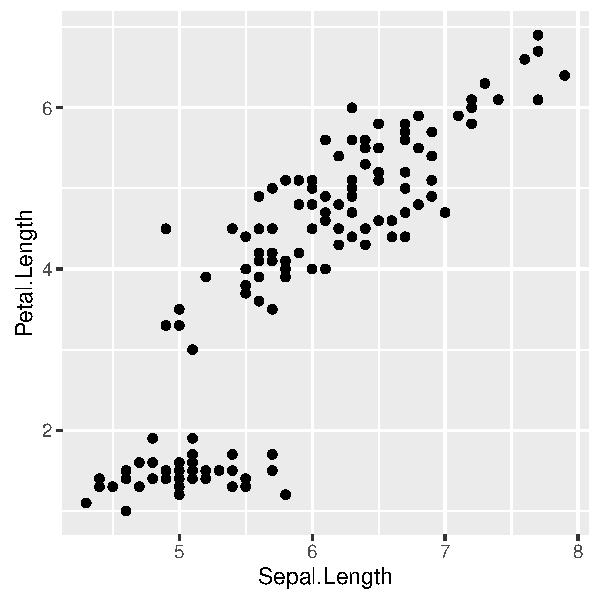
\includegraphics[scale=0.6]{minimal-r17-1.pdf}
					 \label{fig:libro2}
				\end{figure}
				\end{block}

		\end{frame}

	 \begin{frame}[fragile]						% Primera Diapositiva
			\frametitle{Resultado}
		\begin{block}{Sepal.Length vs Petal.Length con color}
					\begin{figure}[htb]
					\centering
					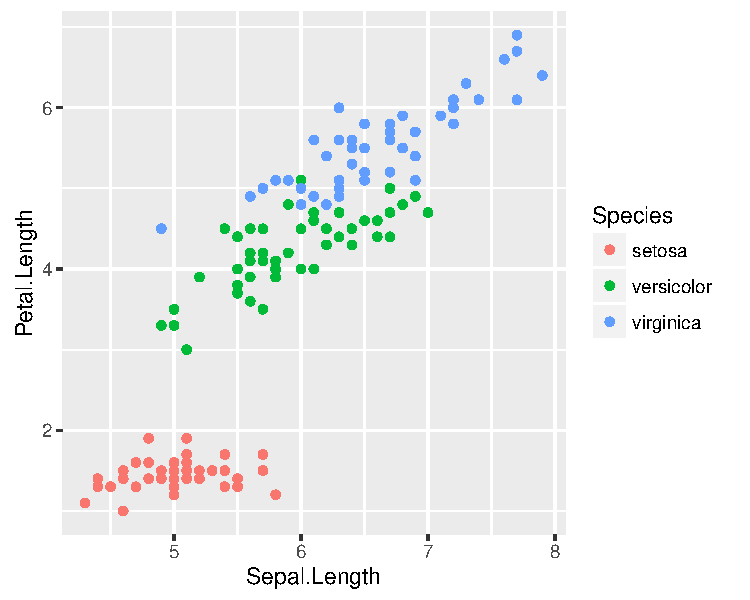
\includegraphics[scale=0.6]{minimal-r18-1.pdf}
					\label{fig:libro3}
				\end{figure}
				\end{block}
		\end{frame}


\section{Bibliografía}	
%BIBLIOGRAFIA 
	\begin{frame}[fragile]
		\frametitle{Bibliografía} 		
        \bibliography{Biblio} 	%Para que aparezca toda la bibliografia que citamos en el documento Biblio.bib, Informe.bbl.
       	\nocite{*}				%Para que aparezca toda la bibliografia que NO citamos en el documento, pero que utilizamos.
	\end{frame}		
				
\end{document}
